\documentclass[]{article}
\usepackage{lmodern}
\usepackage{amssymb,amsmath}
\usepackage{ifxetex,ifluatex}
\usepackage{fixltx2e} % provides \textsubscript
\ifnum 0\ifxetex 1\fi\ifluatex 1\fi=0 % if pdftex
  \usepackage[T1]{fontenc}
  \usepackage[utf8]{inputenc}
\else % if luatex or xelatex
  \ifxetex
    \usepackage{mathspec}
  \else
    \usepackage{fontspec}
  \fi
  \defaultfontfeatures{Ligatures=TeX,Scale=MatchLowercase}
\fi
% use upquote if available, for straight quotes in verbatim environments
\IfFileExists{upquote.sty}{\usepackage{upquote}}{}
% use microtype if available
\IfFileExists{microtype.sty}{%
\usepackage{microtype}
\UseMicrotypeSet[protrusion]{basicmath} % disable protrusion for tt fonts
}{}
\usepackage[margin=1in]{geometry}
\usepackage{hyperref}
\hypersetup{unicode=true,
            pdftitle={MAthesis},
            pdfborder={0 0 0},
            breaklinks=true}
\urlstyle{same}  % don't use monospace font for urls
\usepackage{natbib}
\bibliographystyle{plainnat}
\usepackage{longtable,booktabs}
\usepackage{graphicx,grffile}
\makeatletter
\def\maxwidth{\ifdim\Gin@nat@width>\linewidth\linewidth\else\Gin@nat@width\fi}
\def\maxheight{\ifdim\Gin@nat@height>\textheight\textheight\else\Gin@nat@height\fi}
\makeatother
% Scale images if necessary, so that they will not overflow the page
% margins by default, and it is still possible to overwrite the defaults
% using explicit options in \includegraphics[width, height, ...]{}
\setkeys{Gin}{width=\maxwidth,height=\maxheight,keepaspectratio}
\IfFileExists{parskip.sty}{%
\usepackage{parskip}
}{% else
\setlength{\parindent}{0pt}
\setlength{\parskip}{6pt plus 2pt minus 1pt}
}
\setlength{\emergencystretch}{3em}  % prevent overfull lines
\providecommand{\tightlist}{%
  \setlength{\itemsep}{0pt}\setlength{\parskip}{0pt}}
\setcounter{secnumdepth}{5}
% Redefines (sub)paragraphs to behave more like sections
\ifx\paragraph\undefined\else
\let\oldparagraph\paragraph
\renewcommand{\paragraph}[1]{\oldparagraph{#1}\mbox{}}
\fi
\ifx\subparagraph\undefined\else
\let\oldsubparagraph\subparagraph
\renewcommand{\subparagraph}[1]{\oldsubparagraph{#1}\mbox{}}
\fi

%%% Use protect on footnotes to avoid problems with footnotes in titles
\let\rmarkdownfootnote\footnote%
\def\footnote{\protect\rmarkdownfootnote}

%%% Change title format to be more compact
\usepackage{titling}

% Create subtitle command for use in maketitle
\newcommand{\subtitle}[1]{
  \posttitle{
    \begin{center}\large#1\end{center}
    }
}

\setlength{\droptitle}{-2em}
  \title{MAthesis}
  \pretitle{\vspace{\droptitle}\centering\huge}
  \posttitle{\par}
  \author{}
  \preauthor{}\postauthor{}
  \date{}
  \predate{}\postdate{}

\usepackage{setspace}
\doublespacing

\begin{document}
\maketitle

\begin{longtable}[]{@{}llrrrr@{}}
\caption{Time bins with age range, epoch name, mean age and
corresponding sample sizes (on individual, species and genus
level)}\tabularnewline
\toprule
bin & EpochBins & MeanBins & nIndividuals & nSpecies &
nGenera\tabularnewline
\midrule
\endfirsthead
\toprule
bin & EpochBins & MeanBins & nIndividuals & nSpecies &
nGenera\tabularnewline
\midrule
\endhead
(0,1e-06{]} & Modern & 0.0000005 & 240 & 58 & 17\tabularnewline
(1e-06,0.0117{]} & Holocene & 0.0058500 & 12 & 6 & 4\tabularnewline
(0.0117,0.126{]} & Upper Pleistocene & 0.0688500 & 46 & 15 &
7\tabularnewline
(0.126,0.781{]} & Middle Pleistocene & 0.4535000 & 46 & 9 &
6\tabularnewline
(0.781,2.59{]} & Lower Pleistocene & 1.6845000 & 68 & 24 &
11\tabularnewline
(2.59,3.6{]} & Upper Pliocene & 3.0940000 & 19 & 12 & 8\tabularnewline
(3.6,5.33{]} & Lower Pliocene & 4.4660000 & 23 & 13 & 8\tabularnewline
(5.33,11.6{]} & Upper Miocene & 8.4700000 & 41 & 21 & 9\tabularnewline
\bottomrule
\end{longtable}

\begin{figure}[htbp]
\centering
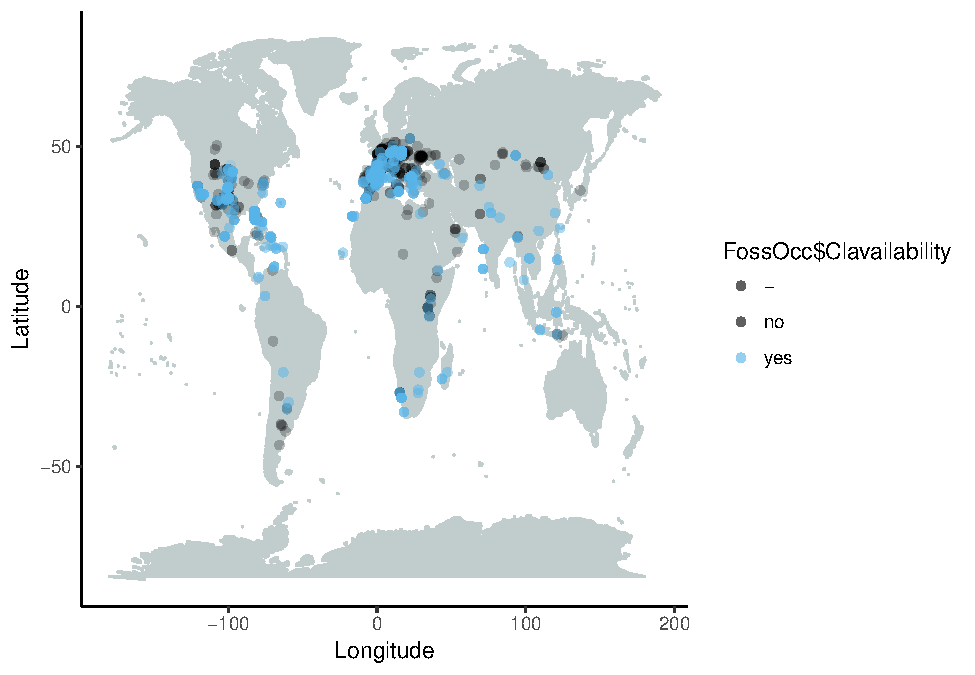
\includegraphics{MA_JJ_files/figure-latex/Map fossil occurrences-1.pdf}
\caption{Map displaying all fossil occurrences of testudinids, with
color indicating whether relevant literature was available (black if
not) and if it was, whether body size data was available or not (yes and
no, respectively).}
\end{figure}

\begin{figure}[htbp]
\centering
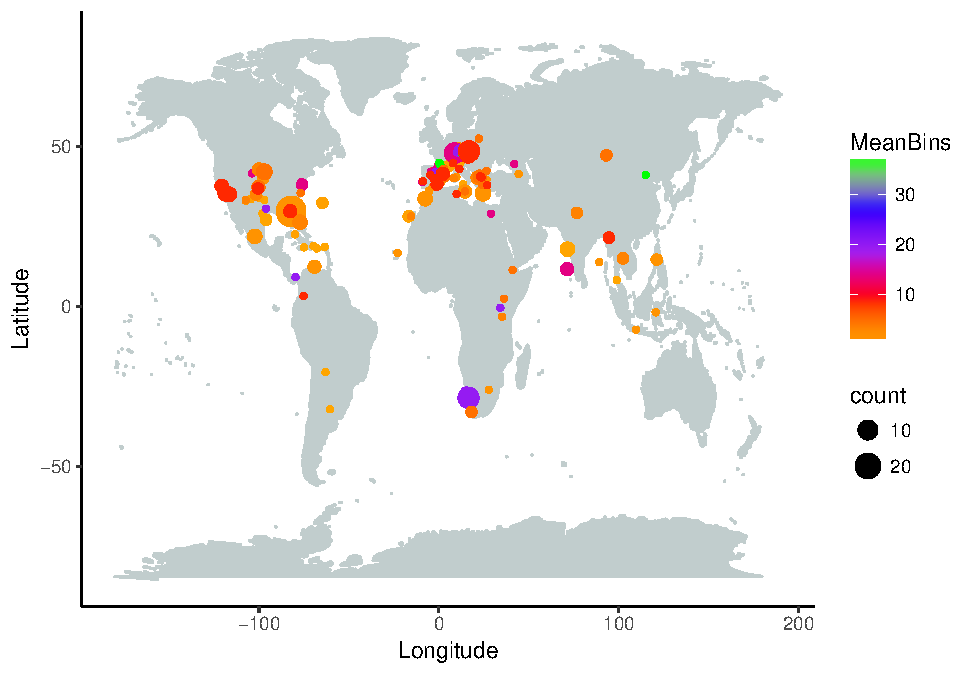
\includegraphics{MA_JJ_files/figure-latex/Map body size data set-1.pdf}
\caption{Map displaying all localities for which body size data for
testudinids was available in the literature. Size of points denotes
sample size, color denotes approximate age.}
\end{figure}

\begin{figure}[htbp]
\centering
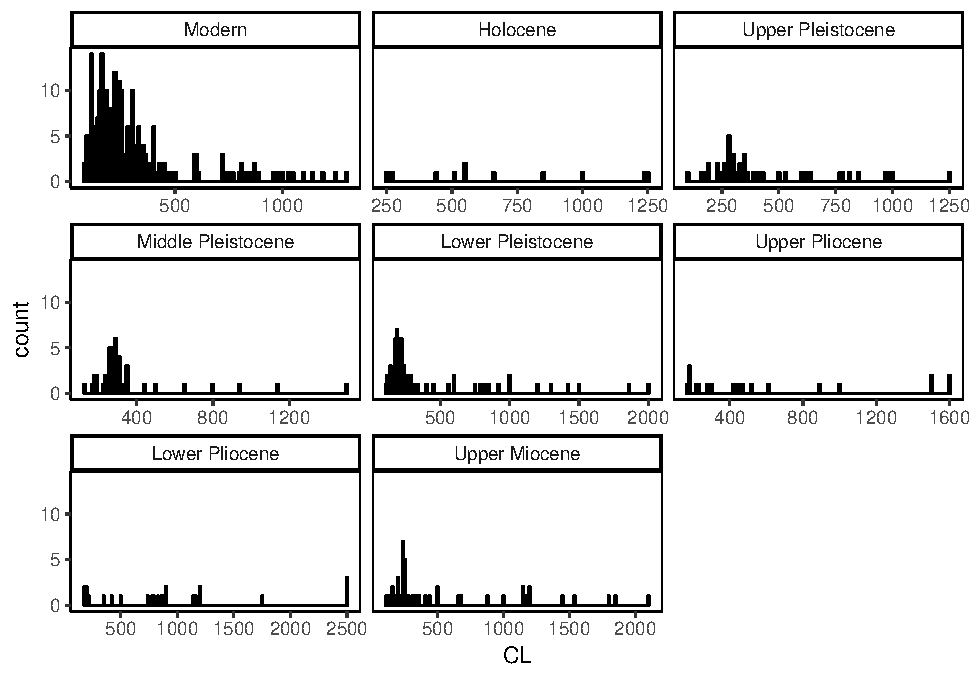
\includegraphics{MA_JJ_files/figure-latex/Histograms of body size data-1.pdf}
\caption{Distribution of body site data per time bin}
\end{figure}

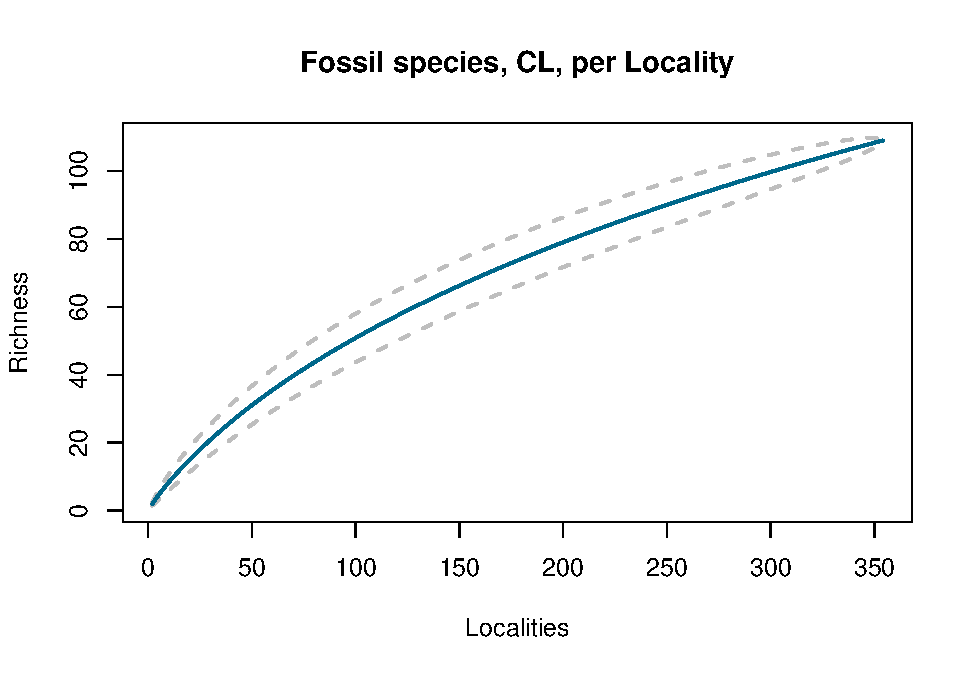
\includegraphics{MA_JJ_files/figure-latex/Species Accumulation Curve-1.pdf}
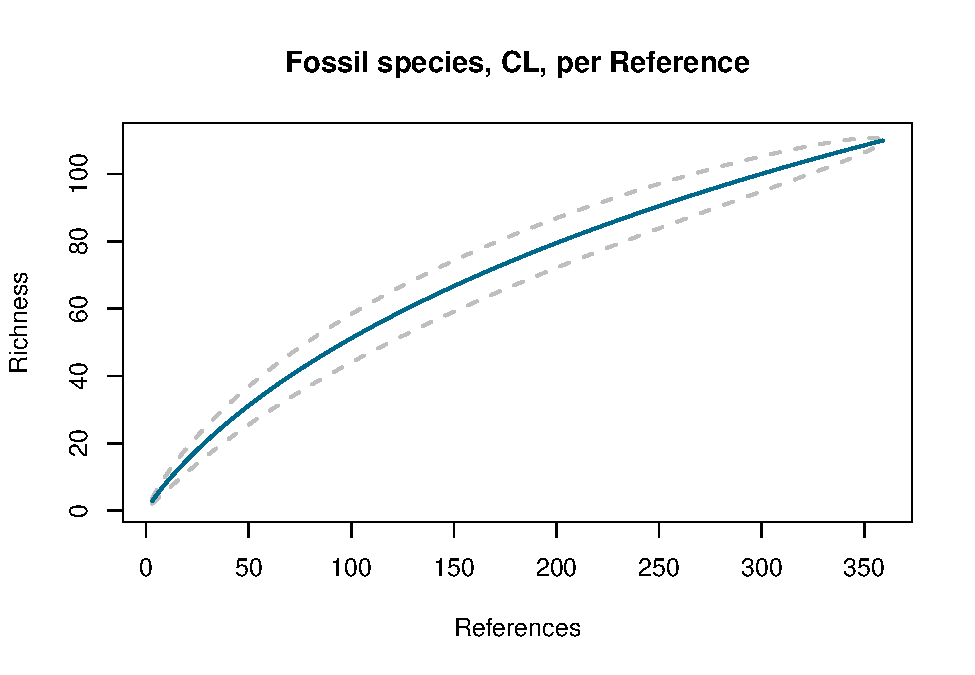
\includegraphics{MA_JJ_files/figure-latex/Species Accumulation Curve-2.pdf}

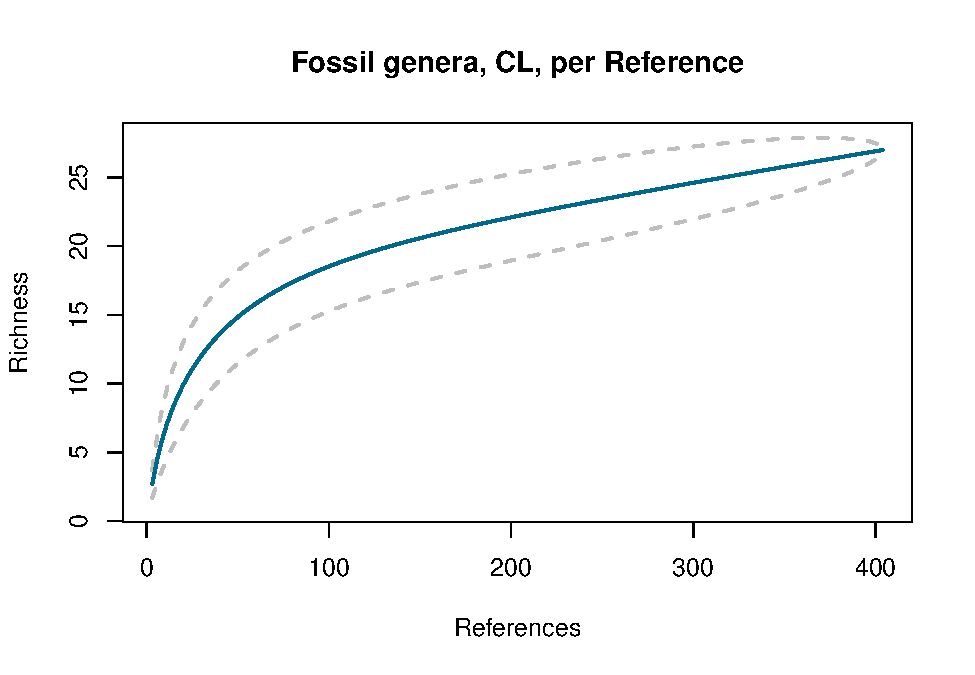
\includegraphics{MA_JJ_files/figure-latex/Species Accumulation Curve with Genera-1.pdf}
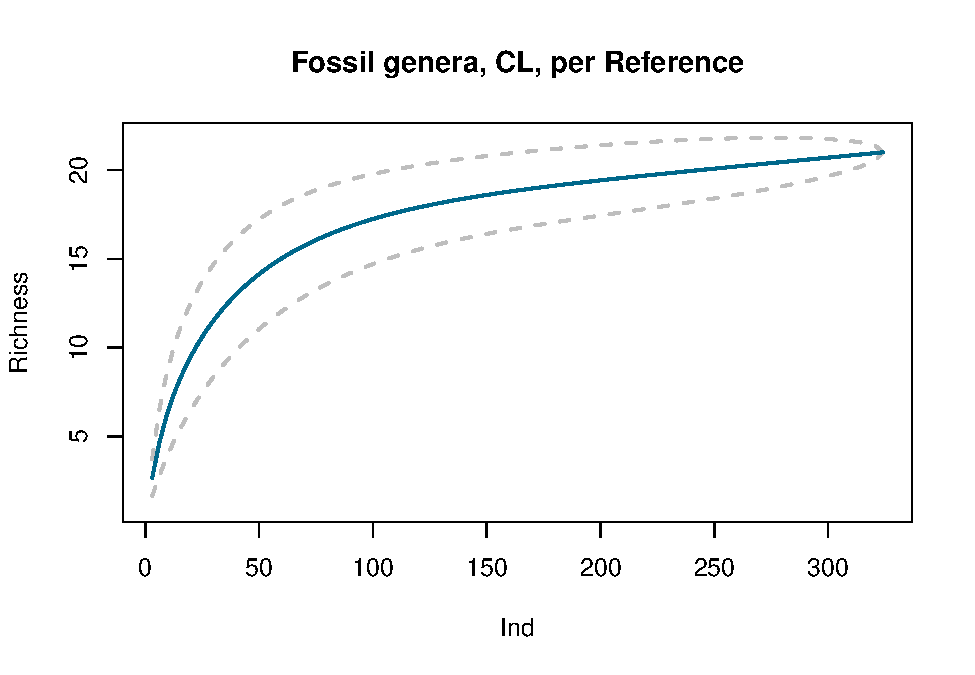
\includegraphics{MA_JJ_files/figure-latex/Species Accumulation Curve with Genera-2.pdf}

\begin{figure}[htbp]
\centering
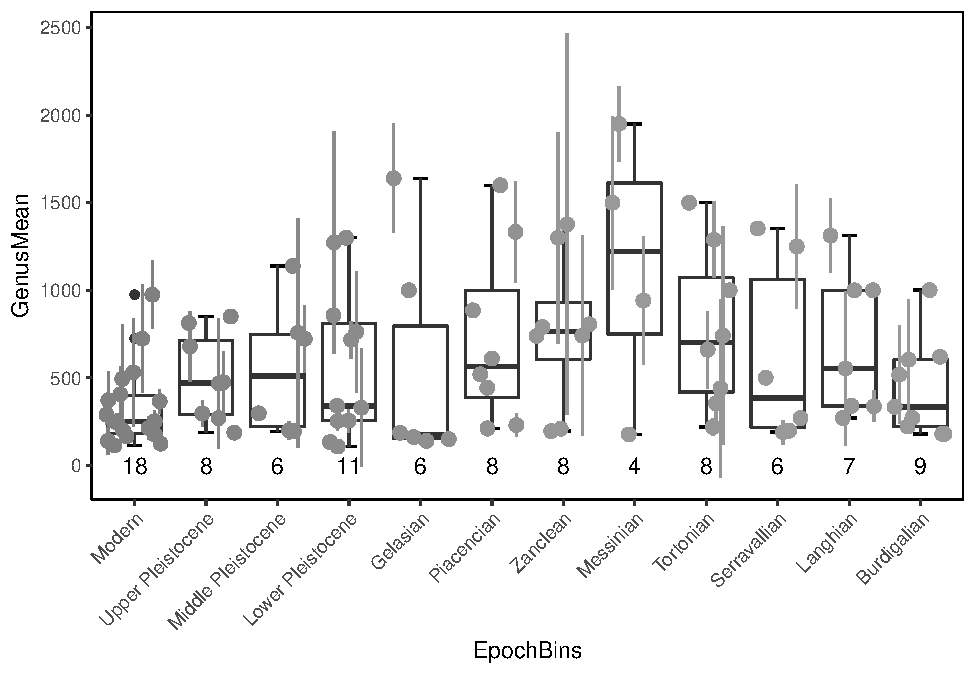
\includegraphics{MA_JJ_files/figure-latex/Boxplots of each genus per time bin-1.pdf}
\caption{Boxplots of each genus per time bin, for colors see Fig. 4.}
\end{figure}

\begin{figure}[htbp]
\centering
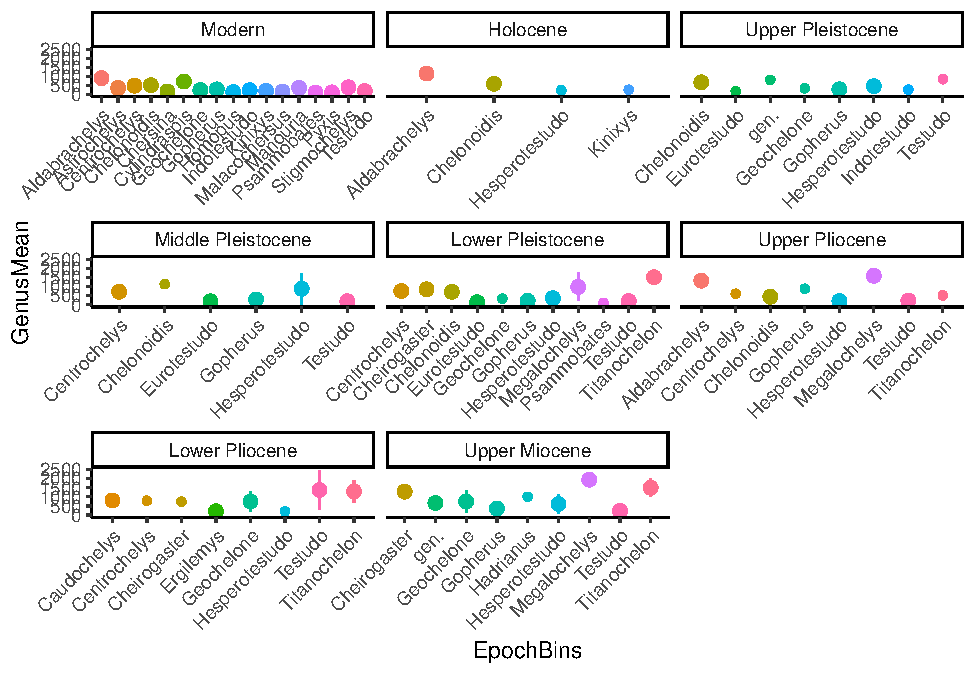
\includegraphics{MA_JJ_files/figure-latex/Separate genera per time bin-1.pdf}
\caption{Mean body size and standard deviation per genus in each time
bin}
\end{figure}

\newpage

\section{including Island species
(n=2215)}\label{including-island-species-n2215}

\begin{figure}[htbp]
\centering
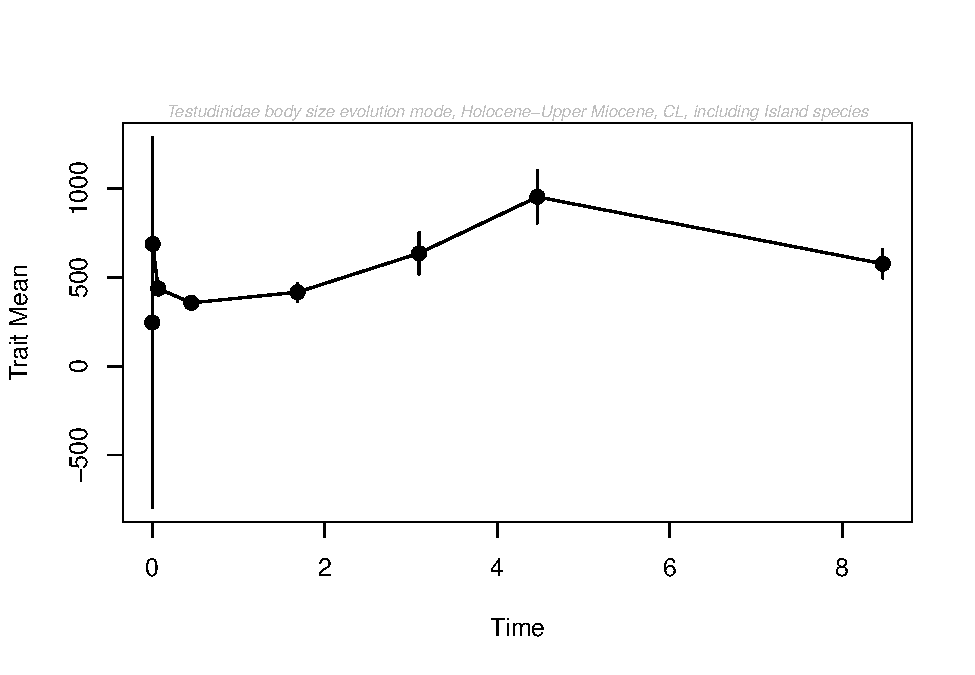
\includegraphics{MA_JJ_files/figure-latex/paleoTS plot-1.pdf}
\caption{individuals, including island species}
\end{figure}

\begin{longtable}[]{@{}lrrrr@{}}
\caption{Model-fitting results for testudinidae, individuals, including
island species}\tabularnewline
\toprule
& logL & K & AICc & Akaike.wt\tabularnewline
\midrule
\endfirsthead
\toprule
& logL & K & AICc & Akaike.wt\tabularnewline
\midrule
\endhead
GRW & -49.84924 & 2 & 106.6985 & 0.044\tabularnewline
URW & -50.76566 & 1 & 104.3313 & 0.145\tabularnewline
Stasis & -46.94604 & 2 & 100.8921 & 0.810\tabularnewline
\bottomrule
\end{longtable}

\newpage

\section{paleoTS plot with species mean, including island
species}\label{paleots-plot-with-species-mean-including-island-species}

\begin{figure}[htbp]
\centering
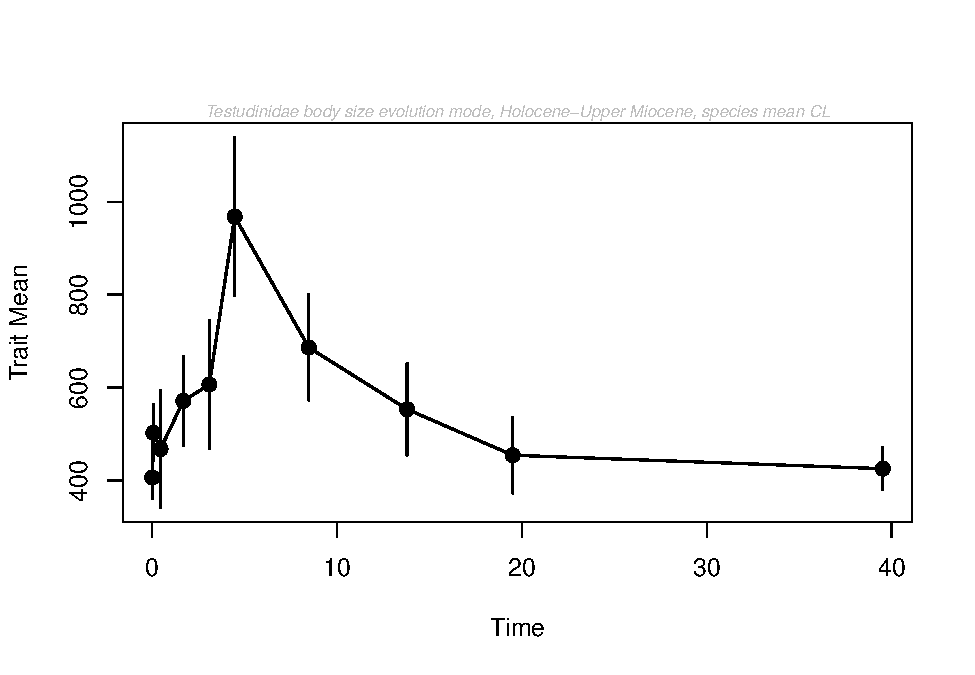
\includegraphics{MA_JJ_files/figure-latex/paleoTS plot with species mean, including island species-1.pdf}
\caption{paleoTS plot with species mean, including island species}
\end{figure}

\begin{longtable}[]{@{}lrrrr@{}}
\caption{Model-fitting results for testudinidae, individuals, including
island species}\tabularnewline
\toprule
& logL & K & AICc & Akaike.wt\tabularnewline
\midrule
\endfirsthead
\toprule
& logL & K & AICc & Akaike.wt\tabularnewline
\midrule
\endhead
GRW & -47.67834 & 2 & 102.35667 & 0.048\tabularnewline
URW & -47.74028 & 1 & 98.28056 & 0.371\tabularnewline
Stasis & -45.19334 & 2 & 97.38669 & 0.580\tabularnewline
\bottomrule
\end{longtable}

\newpage

\section{paleoTS plot with genus
mean}\label{paleots-plot-with-genus-mean}

\begin{figure}[htbp]
\centering
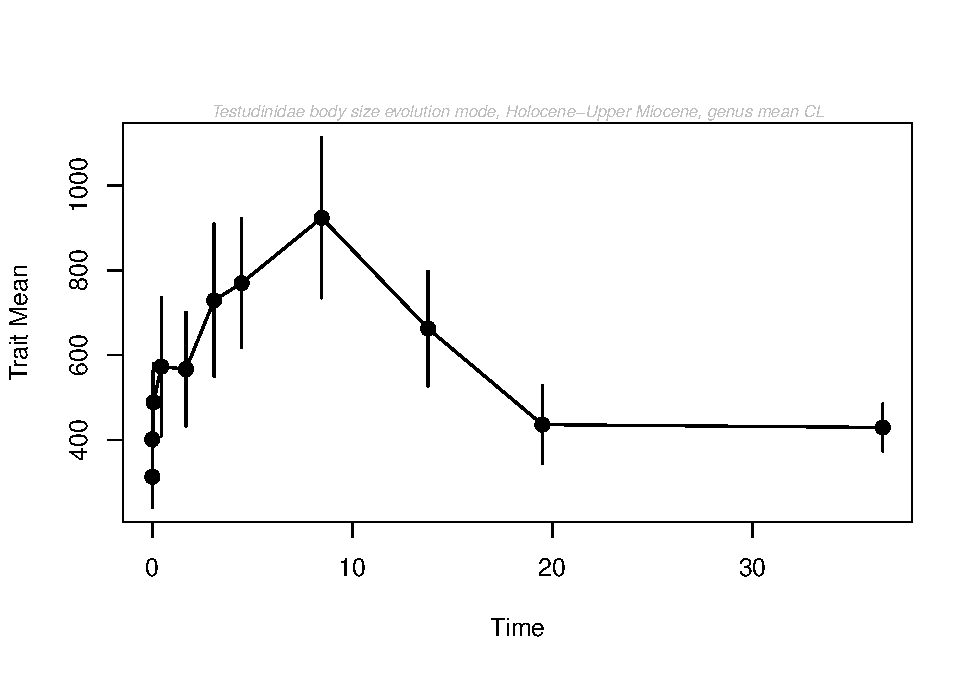
\includegraphics{MA_JJ_files/figure-latex/paleoTS plot with genus mean, including island species-1.pdf}
\caption{paleoTS plot with genus mean, including island species}
\end{figure}

\begin{longtable}[]{@{}lrrrr@{}}
\caption{Model-fitting results for testudinidae, individuals, including
island species}\tabularnewline
\toprule
& logL & K & AICc & Akaike.wt\tabularnewline
\midrule
\endfirsthead
\toprule
& logL & K & AICc & Akaike.wt\tabularnewline
\midrule
\endhead
GRW & -45.37058 & 2 & 97.74116 & 0.107\tabularnewline
URW & -45.58571 & 1 & 93.97143 & 0.702\tabularnewline
Stasis & -44.78886 & 2 & 96.57771 & 0.191\tabularnewline
\bottomrule
\end{longtable}

\newpage

\section{excluding island species}\label{excluding-island-species}

\begin{figure}[htbp]
\centering
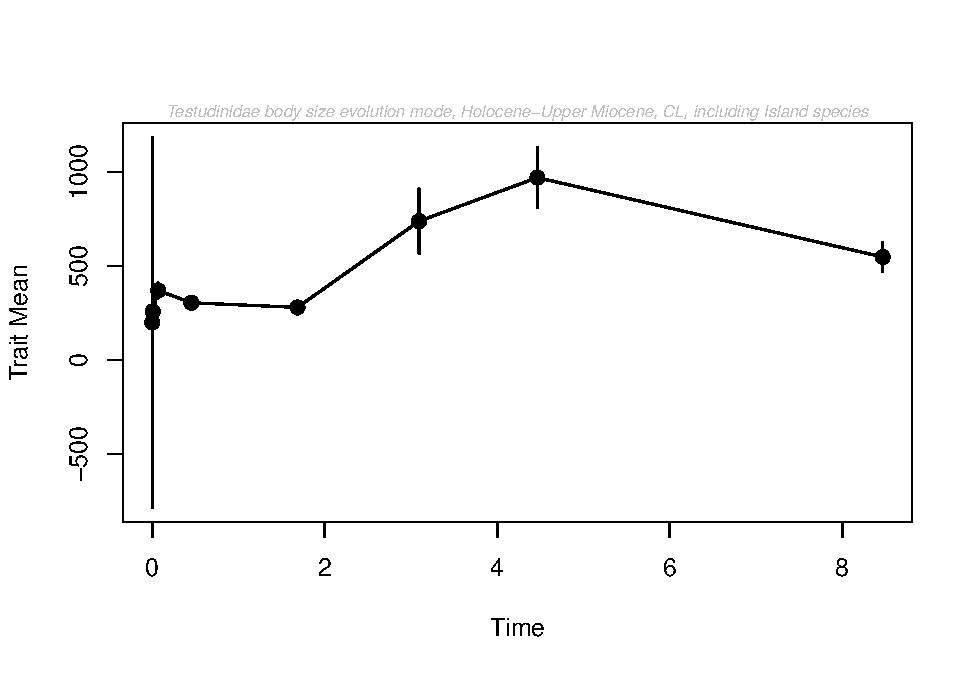
\includegraphics{MA_JJ_files/figure-latex/paleoTS, individuals, exluding island species-1.pdf}
\caption{individuals, excluding island species}
\end{figure}

\begin{longtable}[]{@{}lrrrr@{}}
\caption{Model-fitting results for testudinidae, individuals, including
island species}\tabularnewline
\toprule
& logL & K & AICc & Akaike.wt\tabularnewline
\midrule
\endfirsthead
\toprule
& logL & K & AICc & Akaike.wt\tabularnewline
\midrule
\endhead
GRW & -50.91308 & 2 & 108.8262 & 0.054\tabularnewline
URW & -50.33951 & 1 & 103.4790 & 0.784\tabularnewline
Stasis & -49.81453 & 2 & 106.6291 & 0.162\tabularnewline
\bottomrule
\end{longtable}

\newpage

\section{paleoTS plot with species mean, excluding island
species}\label{paleots-plot-with-species-mean-excluding-island-species}

\begin{figure}[htbp]
\centering
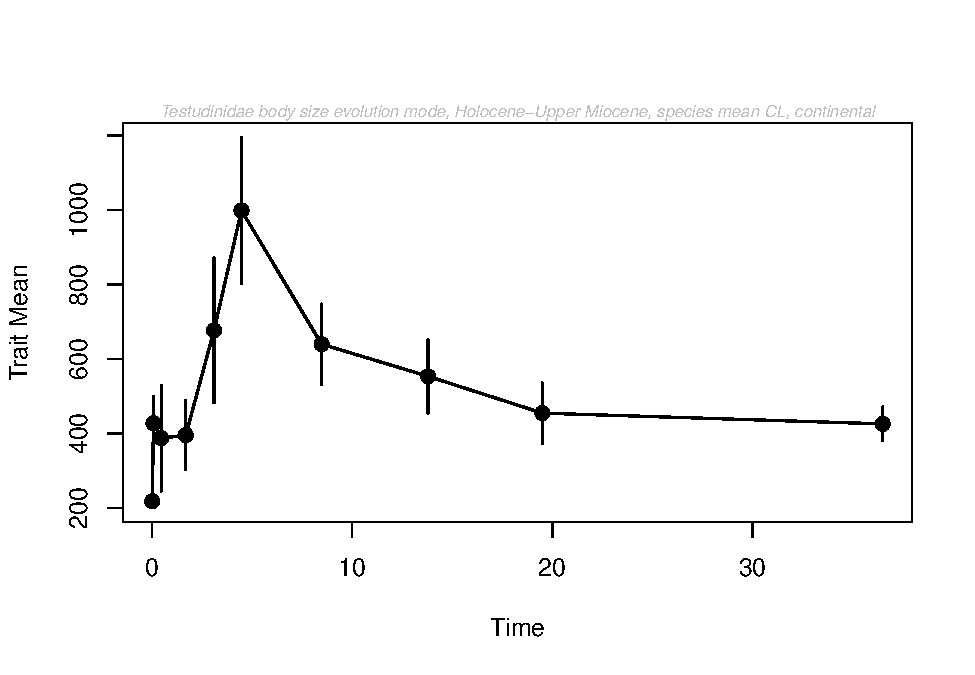
\includegraphics{MA_JJ_files/figure-latex/paleoTS plot with species mean, excluding island species-1.pdf}
\caption{paleoTS plot with species mean, excluding island species}
\end{figure}

\begin{longtable}[]{@{}lrrrr@{}}
\caption{Model-fitting results for testudinidae, individuals, including
island species}\tabularnewline
\toprule
& logL & K & AICc & Akaike.wt\tabularnewline
\midrule
\endfirsthead
\toprule
& logL & K & AICc & Akaike.wt\tabularnewline
\midrule
\endhead
GRW & -48.11009 & 2 & 103.2202 & 0.155\tabularnewline
URW & -48.73586 & 1 & 100.2717 & 0.678\tabularnewline
Stasis & -48.03479 & 2 & 103.0696 & 0.167\tabularnewline
\bottomrule
\end{longtable}

\newpage

\section{paleoTS plot with genus
mean}\label{paleots-plot-with-genus-mean-1}

\begin{figure}[htbp]
\centering
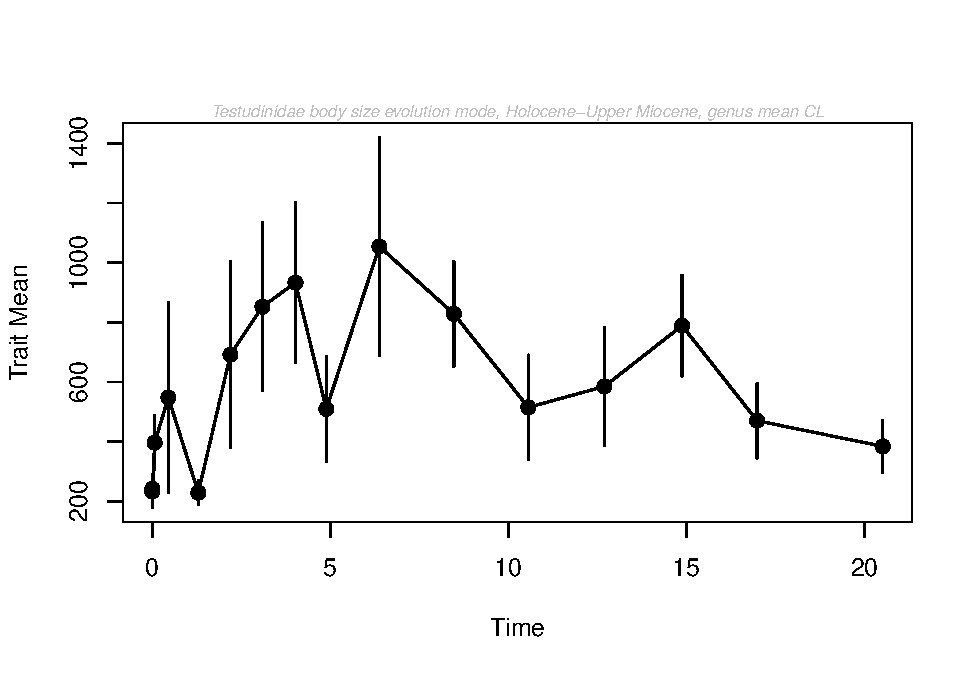
\includegraphics{MA_JJ_files/figure-latex/paleoTS plot with genus mean, excluding island species-1.pdf}
\caption{paleoTS plot with genus mean, excluding island species}
\end{figure}

\begin{longtable}[]{@{}lrrrr@{}}
\caption{Model-fitting results for testudinidae, individuals, including
island species}\tabularnewline
\toprule
& logL & K & AICc & Akaike.wt\tabularnewline
\midrule
\endfirsthead
\toprule
& logL & K & AICc & Akaike.wt\tabularnewline
\midrule
\endhead
GRW & -46.23366 & 2 & 99.46732 & 0.110\tabularnewline
URW & -46.25371 & 1 & 95.30742 & 0.880\tabularnewline
Stasis & -48.57439 & 2 & 104.14878 & 0.011\tabularnewline
\bottomrule
\end{longtable}

\newpage

\section{Boxplots (continental (n) vs.~Island (y)
species)}\label{boxplots-continental-n-vs.island-y-species}

\begin{figure}[htbp]
\centering
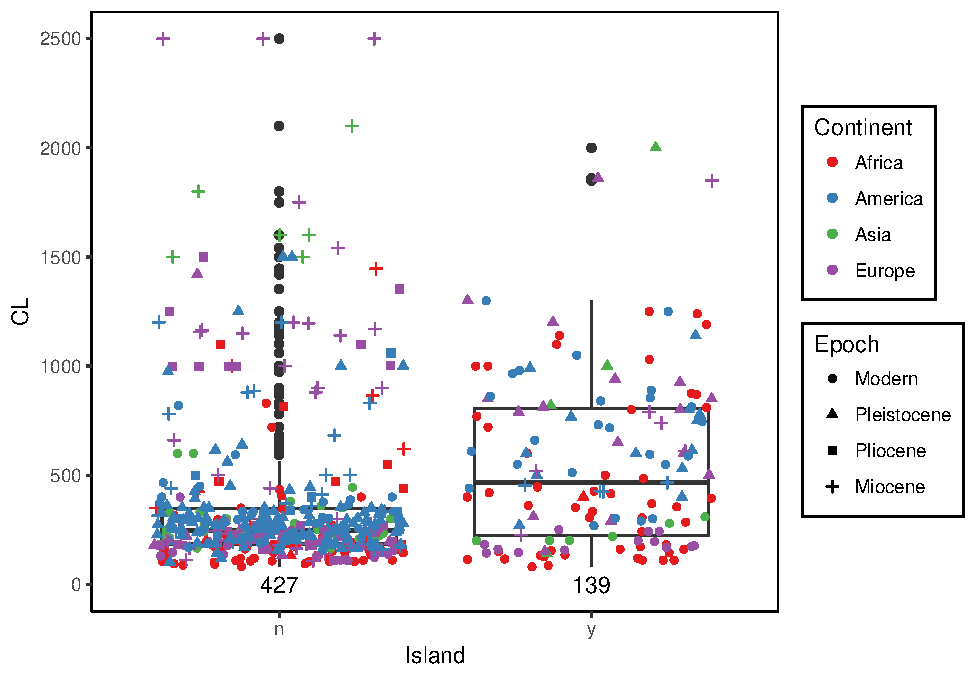
\includegraphics{MA_JJ_files/figure-latex/Boxplot continental vs. insular, individuals-1.pdf}
\caption{Boxplot continental vs.~insular, individuals}
\end{figure}

\begin{figure}[htbp]
\centering
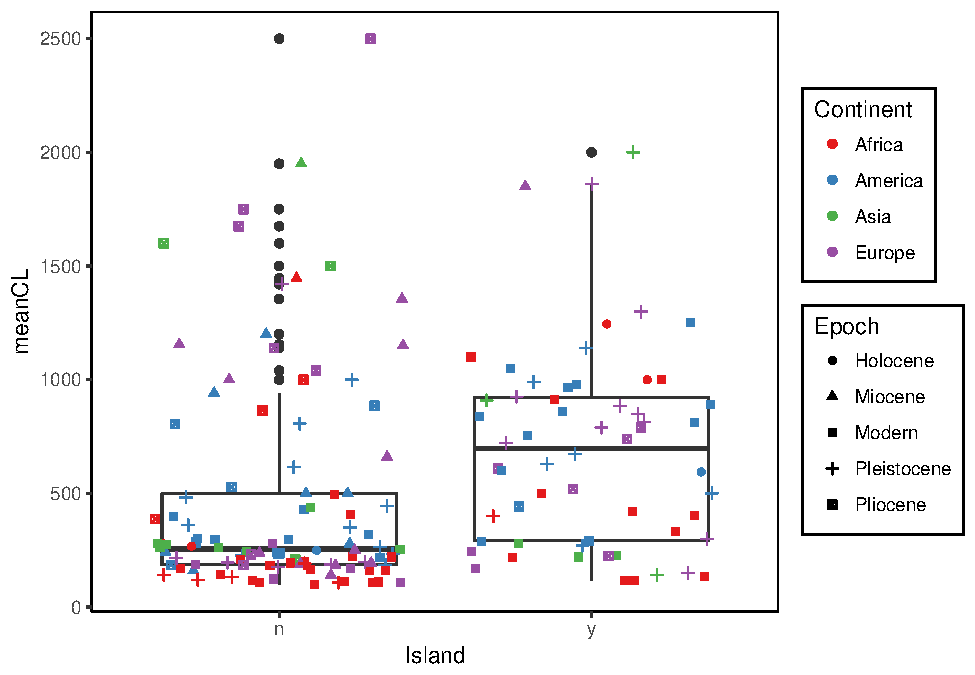
\includegraphics{MA_JJ_files/figure-latex/Boxplots, genera summarised-1.pdf}
\caption{Boxplots continental vs.~insular, genera summarised}
\end{figure}

\begin{figure}[htbp]
\centering
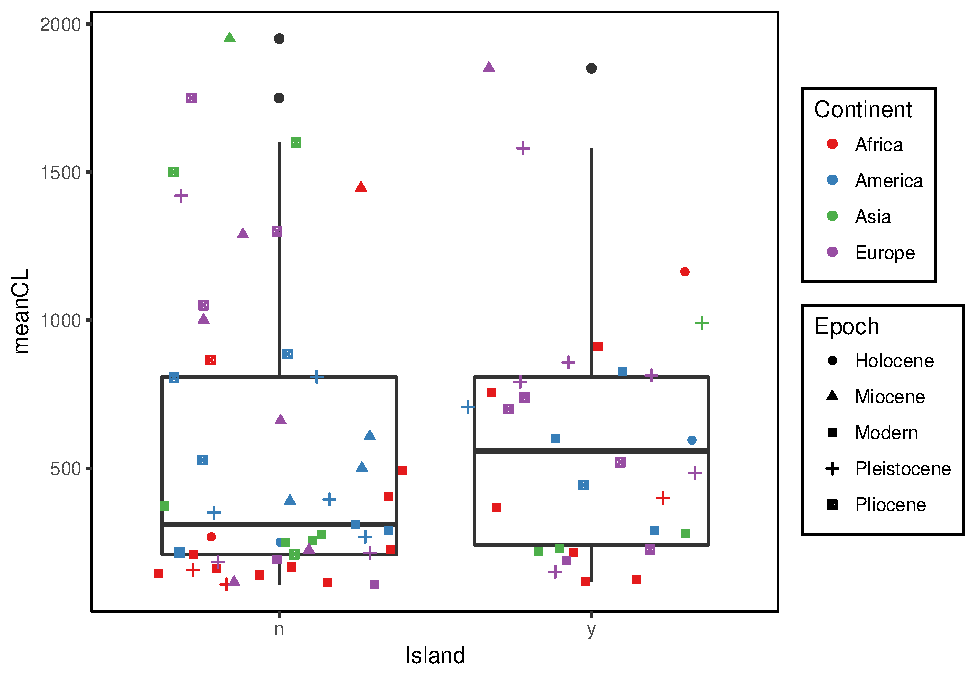
\includegraphics{MA_JJ_files/figure-latex/Boxplot continental vs. insular, species summarised-1.pdf}
\caption{Boxplot continental vs.~insular, species summarised}
\end{figure}

\begin{figure}[htbp]
\centering
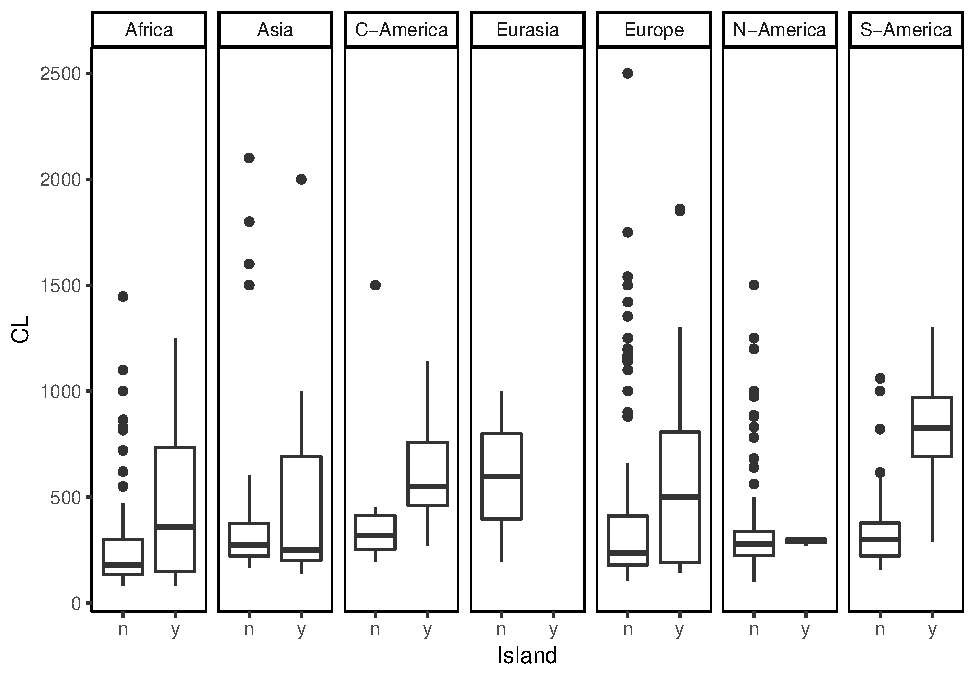
\includegraphics{MA_JJ_files/figure-latex/Boxplots continents, insular vs. continent with age indicated-1.pdf}
\caption{Boxplots of body size (individuals) on different continents,
insular vs.~continent with age indicated}
\end{figure}


\end{document}
